\documentclass[tikz, border=2pt]{standalone}
\usepackage{times}                      
\usepackage[T1]{fontenc}                     
\usepackage{tikz}
\usetikzlibrary{arrows.meta, shapes.geometric, positioning, fit, backgrounds, calc}

\definecolor{traincolor}{RGB}{219, 234, 254}
\definecolor{evalcolor}{RGB}{220, 252, 231}
\definecolor{poolcolor}{RGB}{254, 243, 199}
\definecolor{decisioncolor}{RGB}{243, 232, 255}
\definecolor{borderblue}{RGB}{59, 130, 246}
\definecolor{bordergreen}{RGB}{34, 197, 94}
\definecolor{borderyellow}{RGB}{234, 179, 8}
\definecolor{borderpurple}{RGB}{147, 51, 234}

\tikzset{
  trainbox/.style={
    rectangle, rounded corners=5pt, draw=borderblue, fill=traincolor,
    line width=0.9pt, text width=4.2cm, align=center,
    minimum height=1.0cm, font=\small
  },
  evalbox/.style={
    rectangle, rounded corners=5pt, draw=bordergreen, fill=evalcolor,
    line width=0.9pt, text width=4.2cm, align=center,
    minimum height=1.0cm, font=\small
  },
  poolopbox/.style={
    rectangle, rounded corners=5pt, draw=borderyellow, fill=poolcolor,
    line width=0.9pt, text width=4.2cm, align=center,
    minimum height=1.0cm, font=\small
  },
  decision/.style={
    diamond, aspect=2.8, draw=borderpurple, fill=decisioncolor,
    line width=0.9pt, text width=2.6cm, align=center, font=\small
  },
  poolmember/.style={
    rectangle, rounded corners=3pt, draw=borderyellow, fill=poolcolor,
    line width=0.7pt, text width=2.3cm, align=center,
    minimum height=0.65cm, font=\footnotesize
  },
  arrow/.style={-{Stealth[length=5pt,width=4pt]}, line width=0.8pt},
  dasharrow/.style={-{Stealth[length=5pt,width=4pt]}, line width=0.8pt, dashed},
  lbl/.style={font=\footnotesize, fill=white, inner sep=2pt}
}

\begin{document}
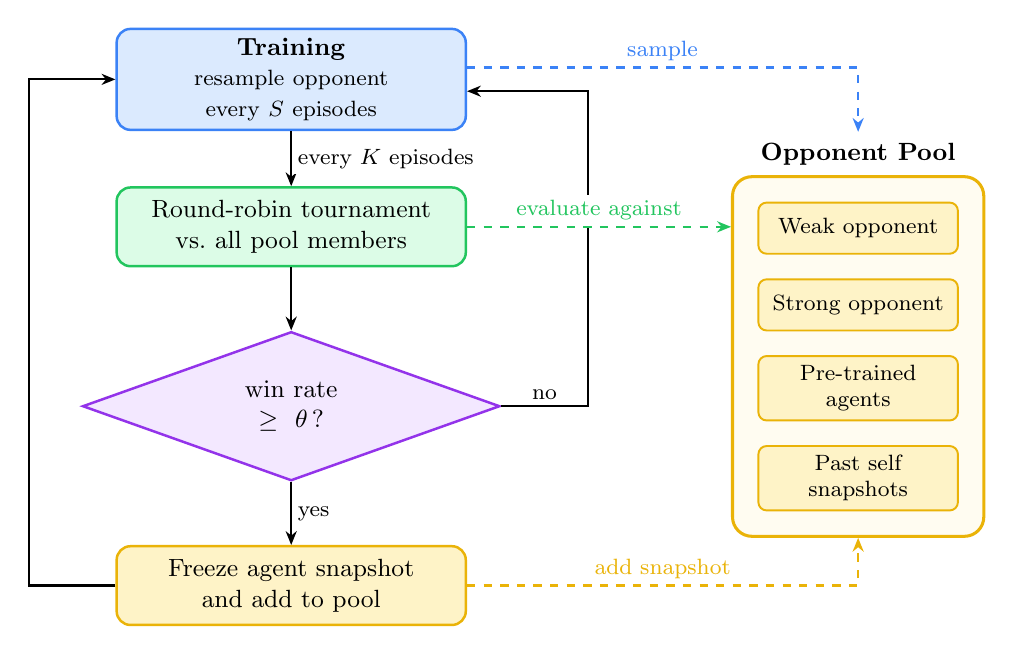
\begin{tikzpicture}[node distance=0.7cm]

  %% ---- Left column ----
  \node[trainbox] (train)
    {\textbf{Training}\\{\footnotesize resample opponent every $S$ episodes}};

  \node[evalbox, below=of train] (eval)
    {Round-robin tournament\\vs.\ all pool members};

  \node[decision, below=of eval, yshift=-0.1cm] (dec)
    {win rate\\$\geq \theta$\,?};

  \node[poolopbox, below=of dec, yshift=-0.1cm] (freeze)
    {Freeze agent snapshot\\and add to pool};

  %% ---- Main downward flow ----
  \draw[arrow] (train) -- node[lbl, right]{every $K$ episodes} (eval);
  \draw[arrow] (eval)  -- (dec);
  \draw[arrow] (dec)   -- node[lbl, right]{yes} (freeze);

  %% ---- "no": exits slightly below train.east, loops back ----
  \draw[arrow] (dec.east)
    -- ++(1.1, 0) node[lbl, above, xshift=-0.55cm]{no}
    |- ([yshift=-0.15cm]train.east);

  %% ---- after freeze: loop back to train (left side) ----
  \draw[arrow] (freeze.west)
    -- ++(-1.1, 0)
    |- (train.west);

  %% ---- Pool members centred on midpoint of left column ----
  \coordinate (leftcol_mid) at ($(train.center)!0.5!(freeze.center)$);

  \node[poolmember] (p1) at ($(leftcol_mid) + (7.2cm, 1.325cm)$)
    {Weak opponent};
  \node[poolmember, below=0.3cm of p1] (p2)
    {Strong opponent};
  \node[poolmember, below=0.3cm of p2] (p3)
    {Pre-trained agents};
  \node[poolmember, below=0.3cm of p3] (p4)
    {Past self snapshots};

  \begin{scope}[on background layer]
    \node[
      rectangle, rounded corners=7pt,
      draw=borderyellow, fill=poolcolor!25,
      line width=1.1pt, inner sep=9pt,
      fit=(p1)(p2)(p3)(p4),
      label={[font=\small\bfseries, anchor=south, name=poollabel]above:Opponent Pool}
    ] (poolouter) {};
  \end{scope}

  %% ---- horizontal centre x of pool ----
  \coordinate (poolcx) at ($(poolouter.west)!0.5!(poolouter.east)$);

  %% ---- blue: clean L-shape, tip points down onto "Opponent Pool" label ----
  \coordinate (poollabelpt) at ($(poolouter.north) + (0, 0.55cm)$);
  \draw[dasharrow, borderblue]
    ([yshift=0.15cm]train.east)
    -- node[lbl, above]{sample} ([yshift=0.15cm]train.east -| poollabelpt)
    -- (poollabelpt);

  %% ---- green: eval --> pool.west (straight across) ----
  \draw[dasharrow, bordergreen]
    (eval.east) -- (poolouter.west |- eval.east)
    node[lbl, midway, above]{evaluate against};

  %% ---- yellow: freeze --> pool.south via horizontal pool centre ----
  \draw[dasharrow, borderyellow]
    (freeze.east)
    -| (poolcx |- poolouter.south)
    node[lbl, near start, above]{add snapshot};

\end{tikzpicture}
\end{document}